\documentclass[11pt,a4paper]{article}

% ---- encoding & fonts ----
\usepackage[T1]{fontenc}
\usepackage[utf8]{inputenc}
\usepackage{lmodern}
\usepackage{microtype}

% ---- layout ----
\usepackage[margin=2.4cm]{geometry}
\usepackage{titlesec}
\usepackage{parskip}

% ---- math ----
\usepackage{amsmath}
\usepackage{amssymb}
\usepackage{bm}

% ---- floats & figures ----
\usepackage{graphicx}
\usepackage{float}
\usepackage{caption}
\usepackage{subcaption}
\usepackage{booktabs}
\usepackage{xcolor}
\graphicspath{{figures/}}

% ---- links ----
\usepackage[hidelinks]{hyperref}
\definecolor{linkblue}{HTML}{2f6df0}
\hypersetup{
  colorlinks=true,
  linkcolor=linkblue,
  citecolor=linkblue,
  urlcolor=linkblue,
}

\titleformat{\section}{\large\bfseries}{\thesection}{0.6em}{}
\titleformat{\subsection}{\normalsize\bfseries}{\thesubsection}{0.6em}{}

\newcommand{\R}{\mathbb{R}}
\emergencystretch=3em

% ---- experiment numbers (filled from report/assets/*.json) ----
\newcommand{\NumEpisodes}{3000}
\newcommand{\NoiseEpisodes}{2400}
\newcommand{\EvalN}{300}
\newcommand{\EvalArrived}{224}
\newcommand{\EvalRate}{74.7\%}
\newcommand{\LateWindowRate}{76.5\%}
\newcommand{\EarlyReturn}{$-$39}
\newcommand{\LateReturn}{$+$97}

\title{\vspace{-1.2cm}\bfseries Learning to Navigate a Mobile Robot in
Randomized Environments with Deep Deterministic Policy Gradients and a
Frontier-Style Exploration Heuristic}
\author{Nikita Sviridov\\\small\texttt{nikswirlo@gmail.com}}
\date{}

\begin{document}
\maketitle

\begin{abstract}
\noindent
We study autonomous point-to-point navigation of a mobile robot in bounded
planar fields cluttered with rectangular obstacles. Unlike a fixed-map
formulation, every training episode samples a fresh task: the number, sizes
and positions of the obstacles and the robot's start pose are all drawn at
random, and a breadth-first search over an inflated occupancy grid certifies
that each sampled layout admits a collision-free corridor to the goal. The
robot perceives its surroundings through a simulated $180^\circ$ lidar and is
driven by a continuous throttle/steering command, which makes the control
problem a natural fit for actor--critic reinforcement learning. We formulate
the task as a Markov decision process, solve it with \emph{Deep Deterministic
Policy Gradient} (DDPG), and augment the agent with a frontier-style
\emph{point-of-interest} (POI) heuristic that turns raw lidar returns into a
compact, goal-directed exploration signal. Trained for \NumEpisodes{} episodes
in minutes on consumer Apple-Silicon hardware, the deterministic policy
reaches the goal on \EvalRate{} of \EvalN{} previously unseen random layouts. Because the map
changes every episode, this figure measures generalization across tasks rather
than the memorization of a single route.
\end{abstract}

\section{Introduction}
Reinforcement learning (RL) has become a standard tool for continuous control,
where the agent must output real-valued commands rather than choose from a
discrete menu of actions~\cite{sutton2018}. Mobile-robot navigation is a
canonical instance: the robot continuously sets its speed and heading to reach a
goal while avoiding collisions, using only local range measurements. Value-based
methods such as DQN~\cite{mnih2015} do not apply directly because the action
space is continuous; deterministic policy gradients~\cite{silver2014} and their
deep counterpart DDPG~\cite{lillicrap2016} close this gap by learning a
parametric actor jointly with a critic.

A policy trained on a single fixed map easily overfits: it can memorize one
route instead of learning to navigate. We therefore train with \emph{domain
randomization} of the layout — every episode presents a new obstacle
configuration and start pose — so the only strategy that survives is one that
reads the lidar and the sub-goal features and reacts to the map it is actually
in.

This report documents an end-to-end navigation system built around DDPG. Our
contributions are: (i) a Markov-decision-process formulation of a lidar-driven
navigation environment (\emph{MobileRobotEnv}) with per-episode layout
randomization and a BFS-certified solvability guarantee; (ii) a frontier-style
POI heuristic that compresses the lidar field into a single goal-directed
sub-target and feeds three scalar features to the policy; (iii) an empirical
study of training dynamics and cross-layout generalization on consumer
hardware; and (iv) a reusable, publication-quality visualisation module for
the environment. All code follows a reproducible \texttt{src}-layout package
with a strict commit-time quality gate.

\section{Problem Formulation}
\subsection{Environment}
The world is an $800 \times 600$ bounded field containing axis-aligned
rectangular obstacles and a fixed goal near the bottom-right corner
(Figure~\ref{fig:env}). At the start of \emph{every} episode the environment
samples a fresh task (Figure~\ref{fig:layouts}):

\begin{itemize}
  \item the \textbf{obstacle count} is drawn uniformly from $\{2,\dots,5\}$;
  \item each obstacle's \textbf{width and height} are drawn uniformly from
        $[60, 220]$ pixels, its position uniformly over the field, rejecting
        overlaps between obstacles and placements that crowd the goal;
  \item the \textbf{start pose} — position and heading
        $\alpha \sim \mathcal{U}[0, 2\pi)$ — is drawn uniformly over the free
        space at least $300$ pixels from the goal.
\end{itemize}

Randomization alone could produce impossible tasks (a wall of obstacles
sealing off the goal). To rule these out, the sampler rasterizes the layout
onto a $20$-pixel occupancy grid, inflates every obstacle by the robot
footprint plus a safety gap, and flood-fills the free cells from the goal by
breadth-first search. Start positions are drawn only from cells connected to
the goal, so \emph{every} sampled task is solvable by construction; layouts
whose free space leaves no valid start cell are resampled.

The robot carries a simulated lidar with seven beams spread uniformly over
$[-90^\circ,+90^\circ]$ relative to its heading; each beam returns the
distance to the nearest obstacle or wall, analytically computed by
ray--rectangle intersection and normalised by the field diagonal
$L=\sqrt{800^2+600^2}$.

\begin{figure}[H]
  \centering
  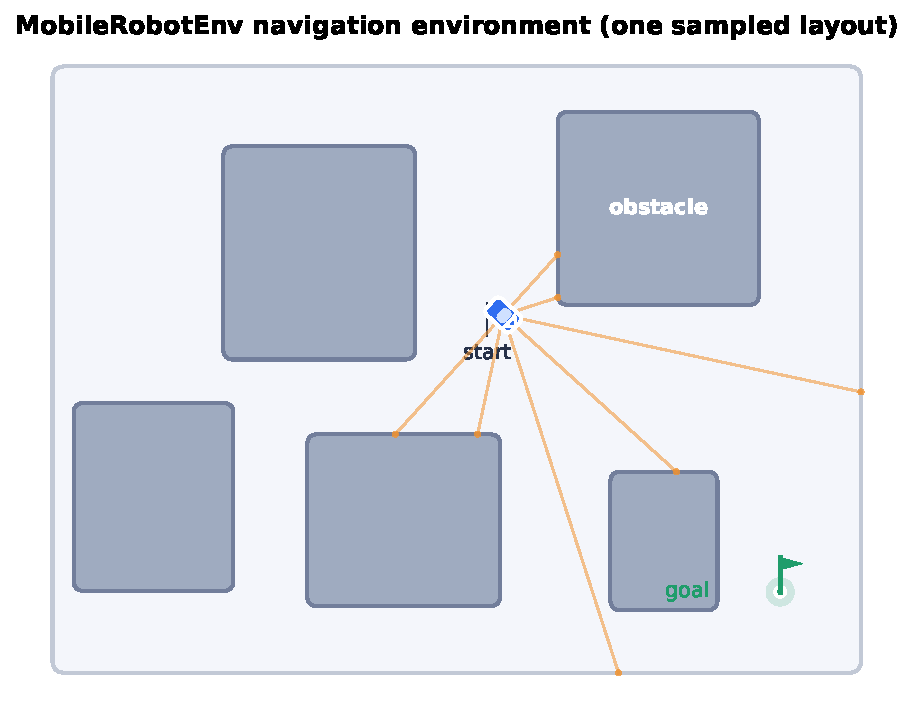
\includegraphics[width=0.82\linewidth]{environment.pdf}
  \caption{The \emph{MobileRobotEnv} environment (one sampled layout). The rover
  (top-down) emits seven lidar beams (orange) that terminate at the nearest
  obstacle or wall. Soft blue blocks are obstacles; the green flag with a
  tolerance halo is the goal.}
  \label{fig:env}
\end{figure}

\begin{figure}[H]
  \centering
  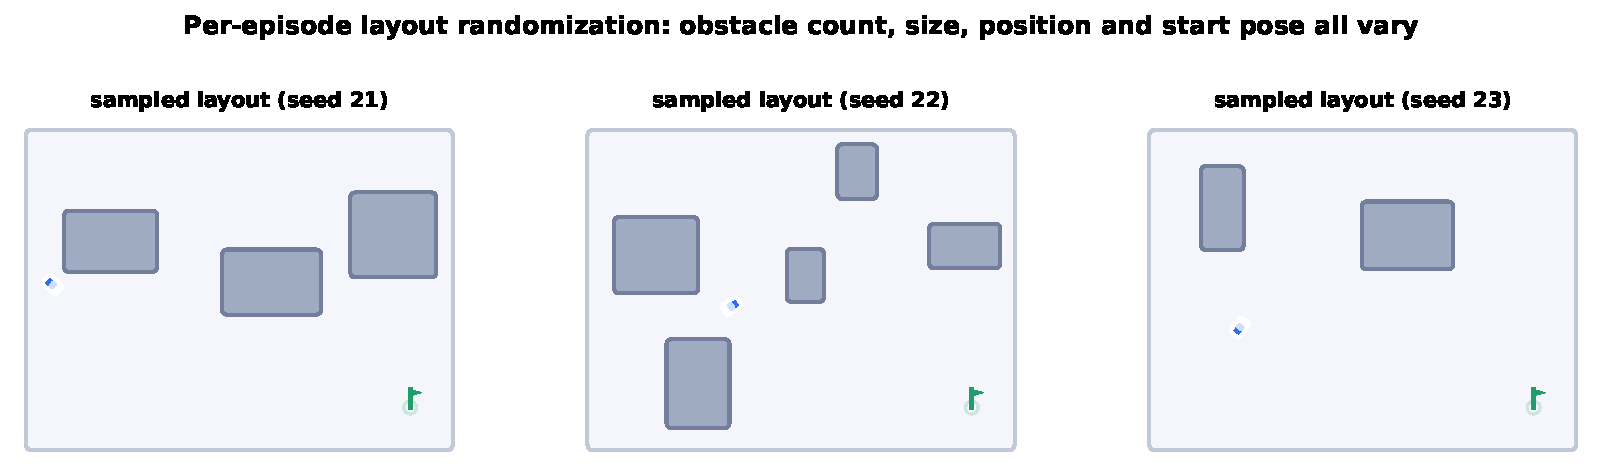
\includegraphics[width=0.98\linewidth]{layouts.pdf}
  \caption{Three independently sampled tasks. Obstacle count, sizes, positions
  and the start pose all vary per episode; a BFS over the inflated occupancy
  grid guarantees a collision-free corridor from every start to the goal.}
  \label{fig:layouts}
\end{figure}

\subsection{Markov decision process}
\paragraph{State $s\in\R^{10}$.}
The observation concatenates the seven normalised lidar ranges
$d_1,\dots,d_7\in[0,1]$ with three goal-directed features derived from the
currently selected POI (Section~\ref{sec:poi}):
\begin{equation}
s = \big(\,d_1,\dots,d_7,\;\tfrac{\theta_{\text{rel}}}{2\pi},\;
\tfrac{\Delta\phi+\pi}{2\pi},\;\tfrac{\rho}{L}\,\big),
\end{equation}
where $\theta_{\text{rel}}$ is the bearing to the POI,
$\Delta\phi \in [-\pi, \pi)$ the \emph{signed} heading error, and $\rho$ the
Euclidean distance to the POI. The sign of $\Delta\phi$ matters: since the
robot's own heading is not part of the observation, an unsigned error would
leave the steering direction unidentifiable — the policy would know how far it
points away from the sub-goal but not which way to turn. On a fixed map this
ambiguity can be compensated by memorizing the route; under layout
randomization it must be resolved in the state itself.

\paragraph{Action $a\in[-1,1]^2$.}
The actor emits a throttle $a_0$ and a steering increment $a_1$ through a
$\tanh$ output. They drive the kinematics
\begin{align}
\alpha &\leftarrow (\alpha + a_1)\bmod 2\pi, &
v &= 10\cdot\tfrac{a_0+1}{2}\in[0,10], \\
x &\leftarrow x + v\cos\alpha, &
y &\leftarrow y + v\sin\alpha.
\end{align}

\paragraph{Reward.}
The agent receives a dense shaping reward that rewards forward speed and
progress toward the goal and penalises turning and time, with large terminal
bonuses/penalties:
\begin{equation}
r =
\begin{cases}
+100 & \text{goal reached } (\rho_g < 10),\\
-50  & \text{collision or out of bounds},\\
a_0 - |a_1| + \kappa\,(\rho_g^{t-1} - \rho_g^{t}) - 1 & \text{otherwise,}
\end{cases}
\end{equation}
with $\kappa = 0.1$. The progress term is potential-based
($\Phi(s) = -\kappa\rho_g$), so it densifies the learning signal without
changing the optimal policy~— important under layout randomization, where the
sparse arrival bonus alone is rarely reached by exploration on a map the agent
has never seen. Episodes terminate on arrival, collision, leaving the field,
or after $500$ steps. Arrival is treated as a terminal transition in the
learning target (no bootstrapping past the goal).

\section{Method}
\subsection{Deep Deterministic Policy Gradient}
DDPG~\cite{lillicrap2016} is an off-policy actor--critic algorithm for
continuous actions. A deterministic actor $\mu_\theta(s)$ proposes an action and
a critic $Q_\psi(s,a)$ estimates its value. The critic minimises the one-step
temporal-difference error against slowly-tracking target networks
$\mu_{\theta'},Q_{\psi'}$:
\begin{align}
y_t &= r_t + \gamma\,(1-\text{done})\,
       Q_{\psi'}\!\big(s_{t+1},\mu_{\theta'}(s_{t+1})\big), \\
\mathcal{L}(\psi) &= \tfrac1N\textstyle\sum_t
       \mathrm{Huber}\big(Q_\psi(s_t,a_t)-y_t\big),
\end{align}
while the actor ascends the critic's value estimate,
$\nabla_\theta J = \tfrac1N\sum_t \nabla_a Q_\psi(s,a)|_{a=\mu_\theta(s)}
\nabla_\theta\mu_\theta(s)$. Target networks are updated by Polyak averaging
$\theta' \leftarrow \tau\theta + (1-\tau)\theta'$. Transitions are stored in a
replay buffer and sampled uniformly to decorrelate updates~\cite{mnih2015}.
Because layouts change per episode, the buffer naturally mixes transitions
from hundreds of distinct maps, which further decorrelates the batches. Both
networks are three-layer perceptrons (Figure~\ref{fig:arch}).

\begin{figure}[H]
  \centering
  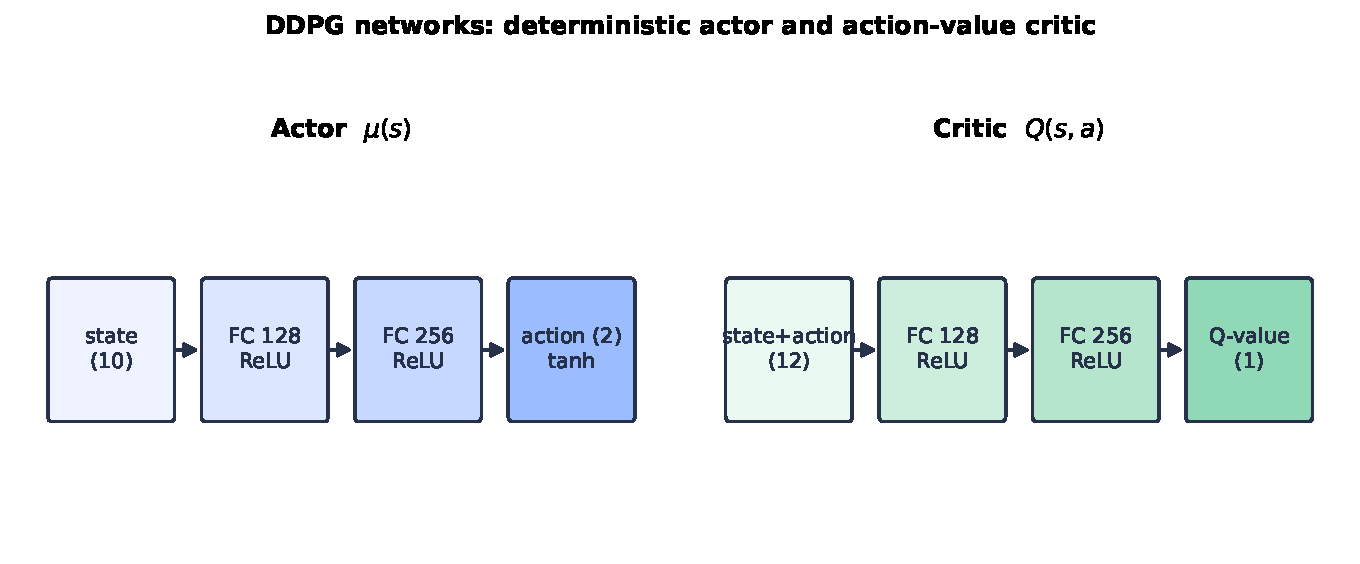
\includegraphics[width=0.98\linewidth]{architecture.pdf}
  \caption{The two DDPG networks. The actor maps a $10$-d state to a $2$-d
  $\tanh$ action; the critic scores a state--action pair ($12$ inputs) with a
  scalar $Q$-value.}
  \label{fig:arch}
\end{figure}

\paragraph{Exploration.}
Because the policy is deterministic, exploration is injected with temporally
correlated Ornstein--Uhlenbeck (OU) noise~\cite{uhlenbeck1930},
$\mathrm{d}x = \theta(\mu - x)\,\mathrm{d}t + \sigma\,\mathrm{d}W$, which
produces smooth, momentum-like perturbations well suited to inertial control.
The noise scale is annealed as $\eta_e=\max(0.1,\,1-e/E_{\text{noise}})$ over
training episode $e$, with $E_{\text{noise}}=\NoiseEpisodes$.

\subsection{Frontier-style POI exploration heuristic}
\label{sec:poi}
Feeding seven raw lidar values to the policy gives only myopic, reactive
information. Inspired by frontier-based exploration~\cite{yamauchi1997}, we
instead distil the lidar field into a single \emph{point of interest}. Along
each free beam we spawn candidate frontier points and score every candidate
$p$ with
\[
\resizebox{\linewidth}{!}{$\displaystyle
h(p) = \underbrace{\tanh\!\Big(
        \tfrac{\exp((d_o/\ell_1)^2)}{\exp((\ell_2/\ell_1)^2)}\Big)\ell_2}
        _{\text{reach / clearance } d_1}
     + \underbrace{d_g}_{\text{goal distance}}
     + \underbrace{\exp(\text{info}/\text{area})}_{\text{information } I}
$}
\]
with $\ell_1=5,\ell_2=20$. The agent selects the candidate of \emph{minimum}
$h$ as its next sub-target; the three POI features above then make the global
goal reachable through a sequence of locally sensible waypoints. Because the
layout is new in every episode, the POI memory (the visited-space field and
the candidate list) is rebuilt from scratch on each reset.
Figure~\ref{fig:poi} visualises $h$ over the free space of one layout: the
basin of low score flows around the obstacles toward the goal.

\begin{figure}[H]
  \centering
  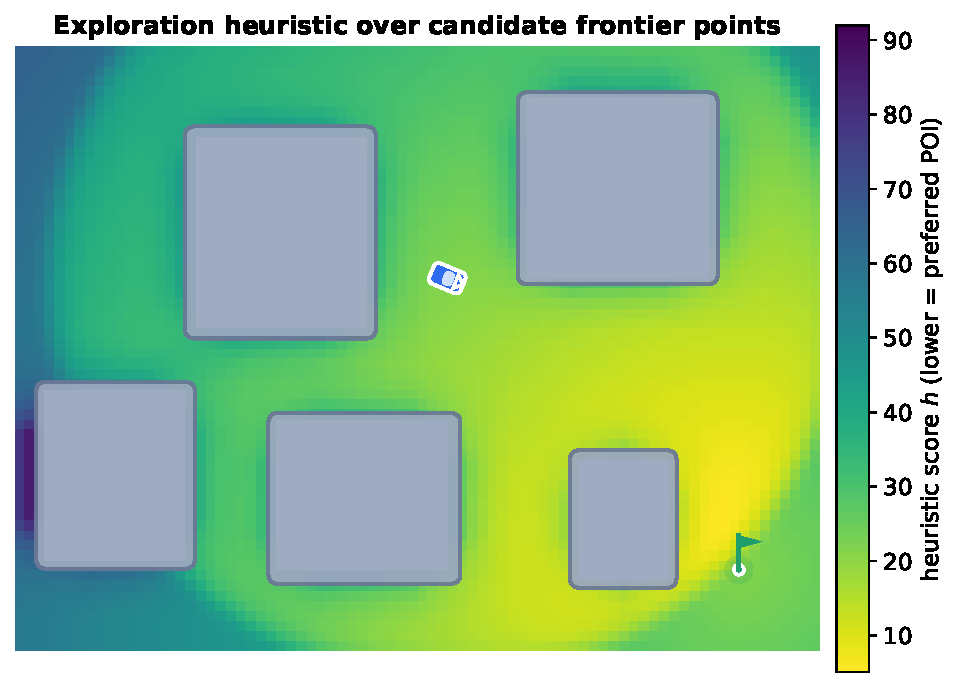
\includegraphics[width=0.82\linewidth]{poi_heatmap.pdf}
  \caption{Exploration heuristic $h$ evaluated over candidate frontier points
  for a rover at the start of one sampled layout. Lower (yellow) is more
  attractive; the field guides sub-target selection around obstacles toward
  the goal.}
  \label{fig:poi}
\end{figure}

\section{Implementation}
The system is implemented in PyTorch as an installable \texttt{src}-layout
package (\texttt{mobile\_robot\_navigation}) with Hydra-based configuration, a
pure-logic training core, and a thin command-line entry point. The layout
randomization is part of the typed environment config (obstacle count and size
ranges, minimum start distance), so sweeps over task difficulty are one-line
Hydra overrides. Device selection prefers CUDA, then Apple MPS, then CPU, so
the same code runs unchanged on a laptop GPU. Quality is enforced at commit
time (Ruff, \texttt{mypy --strict}, property tests, custom style checks);
property-based tests assert the solvability guarantee itself, re-deriving the
BFS corridor check on independently sampled layouts. Table~\ref{tab:hp} lists
the hyperparameters.

\begin{table}[H]
  \centering
  \caption{Training hyperparameters.}
  \label{tab:hp}
  \begin{tabular}{llll}
    \toprule
    Parameter & Value & Parameter & Value\\
    \midrule
    Episodes              & $\NumEpisodes$ & Replay capacity   & $100{,}000$\\
    Max steps / episode   & $500$        & Batch size        & $256$\\
    Discount $\gamma$     & $0.99$       & Actor LR (Adam)   & $1\!\times\!10^{-4}$\\
    Soft-update $\tau$    & $0.005$      & Critic LR (Adam)  & $5\!\times\!10^{-4}$\\
    OU $(\theta,\sigma)$  & $(0.15,0.2)$ & Critic loss       & Huber\\
    Noise episodes        & $\NoiseEpisodes$ & Grad-norm clip    & $1.0$\\
    Hidden units          & $128, 256$   & LR schedule       & linear $\to 0.05$\\
    Obstacles / episode   & $2$--$5$     & Obstacle size     & $60$--$220$ px\\
    \bottomrule
  \end{tabular}
\end{table}

\section{Experiments and Results}
\paragraph{Setup.}
We train for \NumEpisodes{} episodes with a fixed seed on an Apple-Silicon
CPU\footnote{The networks are small enough that the CPU outpaces the MPS
backend, whose per-step host--device synchronisation dominates the step time;
we also observed a deterministic MPS command-buffer hang on long runs.};
every episode runs on a freshly sampled layout. Until the replay buffer holds at
least one batch, actions are sampled uniformly; thereafter the actor acts with
annealed OU noise. For evaluation we roll out the \emph{deterministic} policy
(no exploration noise) on \EvalN{} previously unseen random layouts and report
the goal-arrival rate; during training we also track the per-episode return
and count an episode as an arrival when its return exceeds $50$ (only an
arrival, worth $\approx +94$ net, clears this threshold).

\paragraph{Learning dynamics.}
Figure~\ref{fig:lc} shows the training curves. Thanks to the dense progress
term the agent reaches the goal already in the first hundred episodes
($\sim$$10\%$ of them), and the arrival rate climbs steadily as the noise
anneals, reaching \LateWindowRate{} (true arrivals) over the final $200$
episodes while the mean return rises from \EarlyReturn{} to \LateReturn.
Ablations during development underline how much the task formulation matters
under randomization: with an \emph{unsigned} heading error in the state the
deterministic policy generalized to only $16.7\%$ of unseen layouts, the
signed error lifted it to $31.7\%$, and adding the potential-based progress
term to the reward more than doubled it again.

\begin{figure}[H]
  \centering
  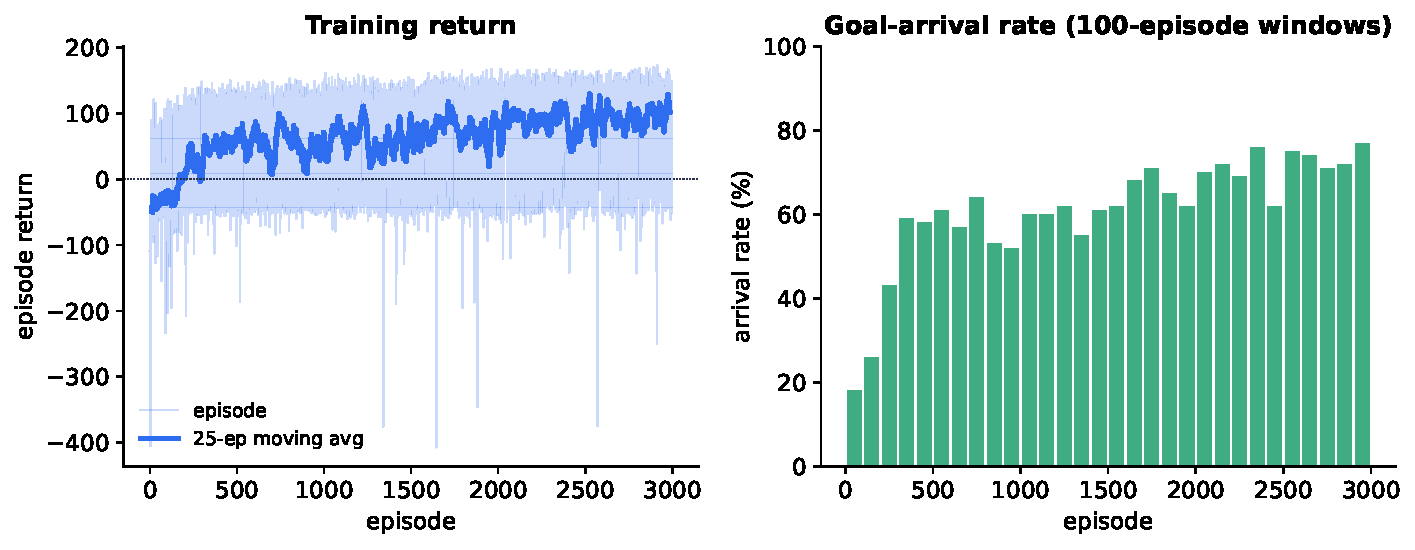
\includegraphics[width=0.98\linewidth]{learning_curve.pdf}
  \caption{Left: per-episode return (faint) with a $25$-episode moving average.
  Right: goal-arrival rate in $100$-episode windows. Every episode is a new
  random layout.}
  \label{fig:lc}
\end{figure}

\paragraph{Generalization across layouts.}
The headline result is the deterministic policy's arrival rate on unseen
tasks: $\EvalArrived/\EvalN$ ($\EvalRate$). Since the evaluation layouts are
sampled from the same distribution but never seen during training, this
directly measures whether the policy learned a navigation \emph{strategy} —
read the lidar, chase the POI sub-goal, avoid what the beams report — rather
than a memorized route. Figure~\ref{fig:traj} shows a successful rollout and a
characteristic failure on two unseen layouts.

\begin{figure}[H]
  \centering
  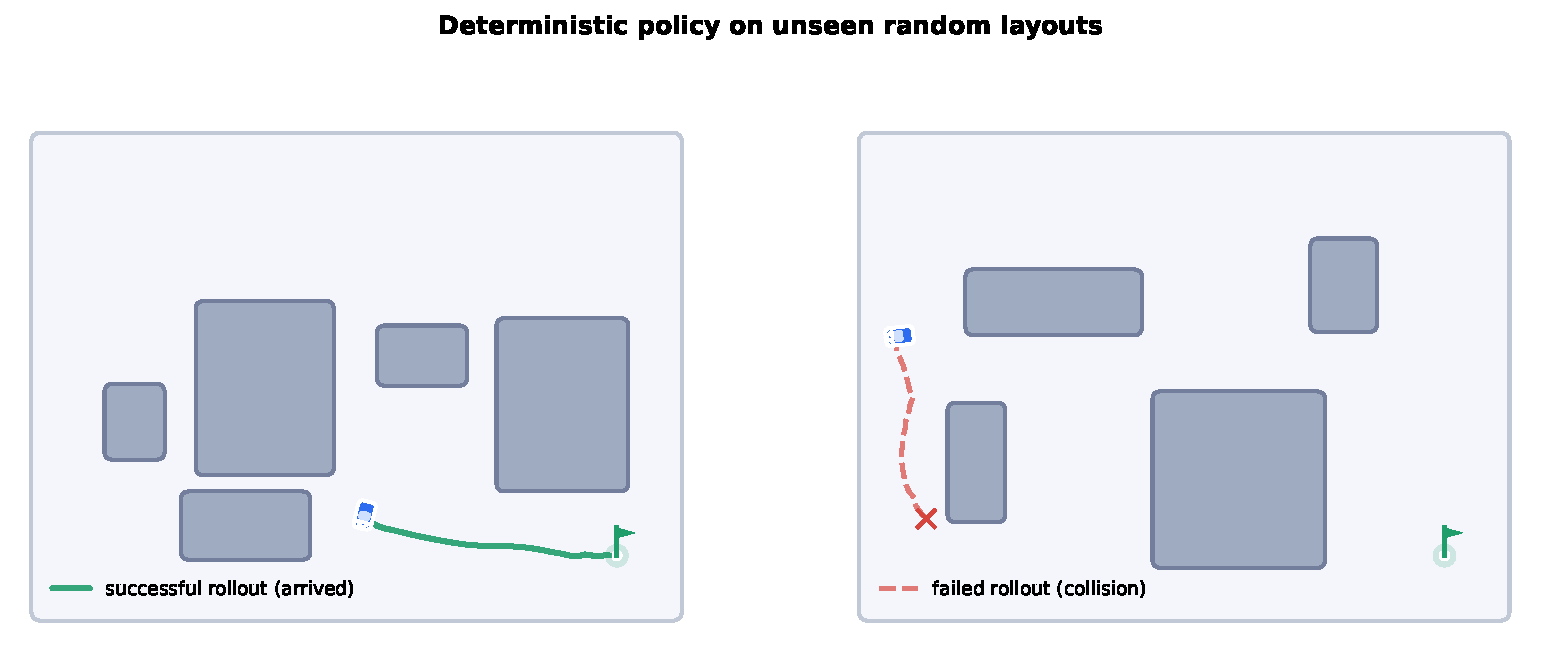
\includegraphics[width=0.98\linewidth]{trajectory.pdf}
  \caption{The deterministic policy on unseen random layouts. Left: a
  successful rollout into the goal halo. Right: a characteristic failure —
  the policy clips an obstacle while cutting a corner.}
  \label{fig:traj}
\end{figure}

\section{Visualisation}
The original environment rendered a raster canvas with bitmap icons. We
replaced it with a vector renderer (\texttt{viz.py}) that draws the field,
rounded obstacles, a goal flag, lidar beams, trajectories, and a stylised
top-down rover with heading and wheels. The same primitives back
\texttt{MobileRobotEnv.render()}, every figure in this report, and an animated
GIF of policy rollouts embedded in the repository README, so the paper and the
live environment are guaranteed to agree. All figures are emitted as scalable
PDF.

\section{Conclusion and Future Work}
We presented a complete DDPG navigation agent trained under per-episode layout
randomization with a BFS-certified solvability guarantee, together with a
frontier-style POI exploration heuristic. On consumer hardware the
deterministic policy generalizes to unseen obstacle layouts with a
\EvalRate{} arrival rate. Natural next steps: TD3-style stabilisation (twin
critics, target-policy smoothing), prioritised replay, randomising the goal
position as well, curriculum over obstacle density, and a learned (rather than
hand-designed) sub-goal proposer.

\begin{thebibliography}{9}
\bibitem{lillicrap2016} T.~P.~Lillicrap, J.~J.~Hunt, A.~Pritzel, et~al.,
``Continuous control with deep reinforcement learning,'' in \emph{ICLR}, 2016.
\bibitem{silver2014} D.~Silver, G.~Lever, N.~Heess, et~al.,
``Deterministic policy gradient algorithms,'' in \emph{ICML}, 2014.
\bibitem{mnih2015} V.~Mnih, K.~Kavukcuoglu, D.~Silver, et~al.,
``Human-level control through deep reinforcement learning,''
\emph{Nature}, vol.~518, pp.~529--533, 2015.
\bibitem{sutton2018} R.~S.~Sutton and A.~G.~Barto,
\emph{Reinforcement Learning: An Introduction}, 2nd ed. MIT Press, 2018.
\bibitem{uhlenbeck1930} G.~E.~Uhlenbeck and L.~S.~Ornstein,
``On the theory of the Brownian motion,''
\emph{Physical Review}, vol.~36, no.~5, pp.~823--841, 1930.
\bibitem{yamauchi1997} B.~Yamauchi,
``A frontier-based approach for autonomous exploration,'' in
\emph{IEEE Int.\ Symp.\ on Computational Intelligence in Robotics and
Automation}, 1997.
\end{thebibliography}

\end{document}
